\documentclass[t,aspectratio=169]{beamer}

\usepackage{soul}
\usepackage{tikz}
\usepackage{multicol}
%\usepackage{gensymb}
\usepackage[utf8]{inputenc}

\usetikzlibrary{arrows.meta,decorations.markings}


%\usepackage{hyperref}
\hypersetup{
    colorlinks=true,
    linkcolor=blue,
    filecolor=magenta,      
    urlcolor=cyan,
    pdftitle={(KTXFI1EBNF) Physics I. Practice},
}

% ----------------------------------------------------------------------------------------------------------------------------------------

\title{\includegraphics[width=45pt]{oepecsetlogo.png}\\(KTXFI1EBNF) Physics I. Practice}

\author{Dr.~Gábor FACSKÓ, PhD\\\tiny Assistant Professor / Senior Research Fellow\\\textit{facsko.gabor@uni-obuda.hu}}

\institute{\Tiny Óbuda University, Faculty of Electrical Engineering, 1084 Budapest, Tavaszmező u. 17.\\Wigner Research Centre for Physics, Department of Space Physics and Space Technology, 1121 Budapest, Konkoly-Thege Miklós út 29–33.\\ \url{https://wigner.hu/~facsko.gabor}}

\date{April~13,~2026}

\logo{\includegraphics[height=0.9 true cm]{kekcsik.png}}

% ----------------------------------------------------------------------------------------------------------------------------------------

\begin{document}

\frame{\titlepage}

% ----------------------------------------------------------------------------------------------------------------------------------------

\begin{frame}[fragile,squeeze,allowframebreaks]
\frametitle{Exercises}
\begin{itemize}
\setlength{\parskip}{0pt}
\setlength{\itemsep}{0pt}
\item \textbf{Thermodynamics I:} Temperature scales, thermal expansion, thermometers. State variables, ideal gas, state changes, ideal gas equation of state, Boyle’s law, Gay-Lussac’s laws, universal (combined) gas law, heat, specific heat, molar heat, heat capacity.
\item \textbf{Thermodynamics II:} Expansion work, internal energy, the first law of thermodynamics, forms of the first law in different state changes.
\item \textbf{Thermodynamics III:} Cyclic processes, Carnot cycle, Carnot’s theorem, reduced heat, entropy, the second law of thermodynamics.
\item \textbf{Thermodynamics IV:} Kinetic theory of gases, molecular thermodynamics. Distributions, distribution functions. Elementary statistics.
\item \textbf{Electrostatics I.:} Electric charge: Fundamental electrical phenomena, electric charge and matter, Coulomb’s law (force between two point charges, unit of electric charge, permittivity of vacuum).

\pagebreak
\item \textbf{Electrostatics II.:} The electric field: The electrostatic field (electric field strength, electric field lines). Determination of electric field strength. Gauss’s law (flux of the electric field). Electric field of a point charge.
  
\pagebreak
\item Problems:
\begin{enumerate}
\setcounter{enumi}{10}   
\item The ideal cycle of an externally heated heat engine, shown in the diagram, differs from the Otto engine cycle in that it contains isothermal processes instead of adiabatic ones.
\vskip -10 pt
\begin{columns}
\begin{column}{0.3\textwidth}
\begin{center}
\vskip -10 pt
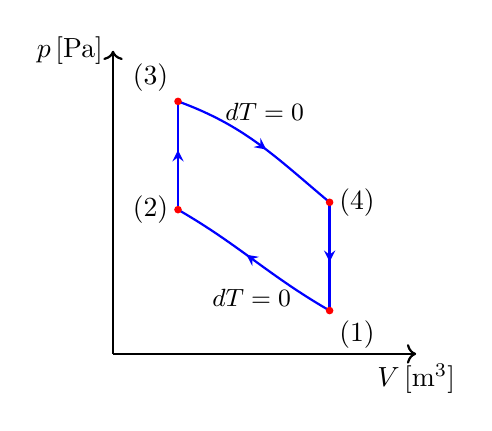
\begin{tikzpicture}[
    % Stílus a vonalak közepén elhelyezett nyilakhoz
    arrow inside/.style={
        postaction={decorate},
        decoration={
            markings,
            mark=at position 0.55 with {\arrow{stealth}}
        }
    }
,scale=0.55]

    % Tengelyek rajzolása feketével, nyilakkal a végén
    \draw[thick, ->] (0,0) -- (7,0) node[below] {$V \, [\mathrm{m^3}]$};
    \draw[thick, ->] (0,0) -- (0,7) node[left] {$p \, [\mathrm{Pa}]$};

    % Pontok koordinátáinak meghatározása
    % Úgy állítjuk be, hogy p3-p2 = p4-p1 legyen (ugyanakkora függőleges szakaszok)
    
    \coordinate (P1) at (5, 1);     % (1) Jobb alsó
    \coordinate (P2) at (1.5, 3.33); % (2) Balra fent (izoterma 1: p*V=5)
    \coordinate (P3) at (1.5, 5.83); % (3) Izochor (p3 = p2 + 2.5)
    \coordinate (P4) at (5, 3.5);    % (4) Izochor (p4 = p1 + 2.5), így p4-p1 = 2.5
    % Megjegyzés: A (3)-(4) görbe így egy másik izoterma (p*V = 1.5*5.83 = 8.75 és 5*3.5 = 17.5)
    % A fizikai hűség kedvéért a (3)-(4) ív is izotermikus marad a rajzon.

    % Folyamatok rajzolása kékkel, középen nyíllal
    % (1) -> (2): Izoterma (dT=0)
    \draw[blue, thick, arrow inside] (P1) to[out=150, in=330] (P2);
    
    % (2) -> (3): Izochor (függőleges, bal oldali)
    \draw[blue, thick, arrow inside] (P2) -- (P3);
    
    % (3) -> (4): Izoterma (dT=0)
    \draw[blue, thick, arrow inside] (P3) to[out=340, in=140] (P4);
    
    % (4) -> (1): Izochor (függőleges, jobb oldali, zárja a kört)
    \draw[blue, thick, arrow inside] (P4) -- (P1);

    % Piros pontok és címkék
    \fill[red] (P1) circle (2.5pt) node[below right, black] {(1)};
    \fill[red] (P2) circle (2.5pt) node[left, black] {(2)};
    \fill[red] (P3) circle (2.5pt) node[above left, black] {(3)};
    \fill[red] (P4) circle (2.5pt) node[right, black] {(4)};

    % Feliratok: dT=0 feketével az izotermák mellett
    \node[black, font=\small] at (3.2, 1.3) {$dT=0$}; 
    \node[black, font=\small] at (3.5, 5.6) {$dT=0$};
\end{tikzpicture}
\end{center}
\end{column}
\begin{column}{0.3\textwidth}
\vfill
What is the efficiency of the cycle if $p_{3} = 4 p_{2}$ , the compression ratio is 6, and the cycle is performed with a two-atomic (diatomic) gas? What is the efficiency of the Carnot cycle taking place between the same temperature limits?
\end{column}
\end{columns}

\bigskip

The ideal cycle of an externally heated heat engine differs from the Otto engine cycle in that it contains isothermal processes instead of adiabatic ones. Calculate:
\begin{enumerate}
    \item[a)] The efficiency ($\eta$) of the cycle if $p_3 = 4p_2$, the compression ratio is $r = 6$, and the gas is diatomic.
    \item[b)] The efficiency of a Carnot cycle ($\eta_{Carnot}$) operating between the same temperature limits.
\end{enumerate}

\begin{itemize}
    \item Pressure ratio: $p_3 = 4p_2$
    \item Compression ratio: $r = \frac{V_1}{V_2} = 6 \implies V_1 = 6V_2$
    \item Gas type: Diatomic (Two-atomic) $\implies C_V = \frac{5}{2}R$
\end{itemize}

\textbf{Efficiency of the Cycle}

\textbf{State (1) to State (2): Isothermal Compression ($T_1 = T_2$)}
According to Boyle-Mariotte's law:
$$ p_1 V_1 = p_2 V_2 \implies p_2 = p_1 \frac{V_1}{V_2} = p_1 \frac{6V_2}{V_2} = 6p_1 $$
The heat released during this process:
$$ Q_{released, 12} = \frac{m}{M} R T_1 \ln\left(\frac{V_2}{V_1}\right) = \frac{m}{M} R T_1 \ln\left(\frac{1}{6}\right) $$

\textbf{State (2) to State (3): Isochoric Heating ($V_2 = V_3$)}
According to Gay-Lussac's II law:
$$ \frac{p_2}{T_2} = \frac{p_3}{T_3} \implies \frac{T_3}{T_2} = \frac{p_3}{p_2} = 4 \implies T_3 = 4T_2 = 4T_1 $$
The heat absorbed during this process:
$$ Q_{absorbed, 23} = C_V \frac{m}{M} (T_3 - T_2) = \frac{5}{2} R \frac{m}{M} (4T_1 - T_1) = \frac{15}{2} R \frac{m}{M} T_1 $$

\textbf{State (3) to State (4): Isothermal Expansion ($T_3 = T_4$)}
Since $T_3 = T_4 = 4T_1$ and $V_4 = V_1, V_3 = V_2$:
$$ Q_{absorbed, 34} = \frac{m}{M} R T_3 \ln\left(\frac{V_4}{V_3}\right) = \frac{m}{M} R (4T_1) \ln\left(\frac{6V_2}{V_2}\right) = \frac{m}{M} R T_1 \cdot 4 \ln 6 $$

\textbf{State (4) to State (1): Isochoric Cooling ($V_4 = V_1$)}
The heat released during this process:
$$ Q_{released, 41} = C_V \frac{m}{M} (T_1 - T_4) = \frac{5}{2} R \frac{m}{M} (T_1 - 4T_1) = -\frac{15}{2} R \frac{m}{M} T_1 $$

\textbf{Efficiency Calculation:}
The efficiency is defined as $\eta = \frac{\sum Q}{Q_{absorbed, total}}$.
The total absorbed heat is $Q_{absorbed} = Q_{23} + Q_{34}$.
The net heat is $\sum Q = Q_{12} + Q_{23} + Q_{34} + Q_{41}$.
$$ \eta = \frac{\frac{m}{M} R T_1 \ln(\frac{1}{6}) + \frac{15}{2} R \frac{m}{M} T_1 + \frac{m}{M} R T_1 \cdot 4 \ln 6 - \frac{15}{2} R \frac{m}{M} T_1}{\frac{15}{2} R \frac{m}{M} T_1 + \frac{m}{M} R T_1 \cdot 4 \ln 6} $$
Simplifying by $\frac{m}{M} R T_1$:
$$ \eta = \frac{-\ln 6 + 4 \ln 6}{7.5 + 4 \ln 6} = \frac{3 \ln 6}{7.5 + 4 \ln 6} \approx \frac{5.375}{14.667} \approx 0.3665 $$
$$ \mathbf{\eta = 36.65\%} $$

\pagebreak
\textbf{Carnot Efficiency}
The Carnot efficiency between $T_H = 4T_1$ and $T_L = T_1$:
$$ \eta_{Carnot} = \frac{T_H - T_L}{T_H} = \frac{4T_1 - T_1}{4T_1} = \frac{3}{4} = 0.75 $$
$$ \mathbf{\eta_{Carnot} = 75\%} $$

\end{enumerate}

\end{itemize}

\end{frame}

% ----------------------------------------------------------------------------------------------------------------------------------------

\begin{frame}
%\frametitle{Minden jó, ha a vége jó}

\vfill
\begin{center}
\textbf{\huge The End}

\bigskip
Thank you for your attention!
\end{center}
\vfill
%\textbf{Acknowledgements} Thank you for the course materials for Szilárd~ZSÓKA and Zoltán~VARGA.
\end{frame}

\end{document}
